
%\documentclass[submit]{ipsj}
%\documentclass[submit,draft]{ipsj}
\documentclass[submit,techreq,noauthor]{ipsj}

\usepackage[dvips]{graphicx}
\usepackage{latexsym}

\def\Underline{\setbox0\hbox\bgroup\let\\\endUnderline}
\def\endUnderline{\vphantom{y}\egroup\smash{\underline{\box0}}\\}
\def\|{\verb|}

%%%%%%%%%%%%%%%%%%%%%%%%%%%%%%%%%%%%%%%%%%%%%%%%%%%%%%%%%%%%%%%%
\bibliographystyle{ipsjsort}
%\usepackage{listings,jlisting}
\usepackage{listings}
\newcommand{\myvec}[1]{\vec{#1}}
\newcommand{\araa}{Annual Review of Astronomy and Astrophysics}
\newcommand{\icarus}{Icarus}
\newcommand{\mnras}{Monthly Notices of the Royal Astronomical Society}
\newcommand{\apj}{Astrophysical Journal}
\newcommand{\pasa}{Publications of the Astronomical Society of Australia}
\newcommand{\pasj}{Publications of the Astronomical Society of Japan}
\newcommand{\aap}{Astronomy and Astrophysics}
%%%%%%%%%%%%%%%%%%%%%%%%%%%%%%%%%%%%%%%%%%%%%%%%%%%%%%%%%%%%%%%%

\setcounter{巻数}{53}
\setcounter{号数}{10}
\setcounter{page}{1}

\受付{2011}{11}{4}
%\再受付{2011}{7}{16}   %省略可能
%\再再受付{2011}{7}{20} %省略可能
\採録{2011}{12}{1}

\begin{document}


\title{FDPS(Framework for Developing Particle Simulator): \\ 大規模分散メ
  モリー環境下での粒子系シミュレーション用フレームワークの開発}

%\etitle{How to Prepare Your Paper for IPSJ Journal \\
%(version 2012/10/12)}

\affiliate{RIKEN}{理化学研究所 計算科学研究機構\\
  RIKEN Advanced Institute for Computational Science}

\affiliate{TITEC}{東京工業大学\\
Tokyo Institute of Technology}

\author{岩澤 全規}{Masaki Iwasawa}{RIKEN}[masaki.iwasawa@riken.jp]
\author{谷川 衝}{Ataru Tanikawa}{RIKEN}[ataru.tanikawa@riken.jp]
\author{細野 七月}{Natsuki Hosono}{RIKEN}[natsuki.hosono@riken.jp]
\author{似鳥 啓吾}{Keigo Nitadori}{RIKEN}[keigo@riken.jp]
\author{村主 崇行}{Takayuki Muranushi}{RIKEN}[takayuki.muranushi@riken.jp]
\author{牧野 淳一郎}{Junichiro Makino}{RIKEN,TITEC}[jmakino@riken.jp]

\begin{abstract}
  
粒子法を用いたシミュレーションは科学や工学の幅広い分野で広く使われてお
り,使用されるアルゴリズムも似ている.しかし,今までのソフトウェアは各
分野で独立に開発されており,分野間で共用する事は難しかった.一方,「京」
の様な大規模並列型スパコンで効率よく動作する粒子法プログラムの開発は容
易ではなく,多くの研究者はソフトウェアの開発に多大な時間と労力を割いて
いる.そこで,本研究では,「京」の様な大規模並列型スパコンで効率よく動
作する粒子法シミュレーションプログラムをユーザーが容易に開発できるフレー
ムワーク(FDPS: Framework for DevelopingParticle Simulator)を開発した.
粒子法の大規模並列プログラムが複雑になるのは,計算領域分割やその領域に
合わせた粒子の再配分,また効率的な相互作用のために必要な粒子のツリー構
造での管理等が必要なためである.FDPSはこの部分を担当する.そのため,ユー
ザーは並列化を意識することなくプログラムの開発を行うことができる.我々
は,実際にFDPSを使ったいくつかのプログラムの開発も行い,「京」などのス
パコンで実行した.その結果,プログラムが数百行で書け,また非常に高い実
行効率が出る事を確認した.
  
\end{abstract}

\begin{jkeyword}
粒子法,HPC,MPI+OpenMP並列
\end{jkeyword}

%\begin{eabstract}
%This document is a guide to prepare a draft for submitting to IPSJ
%Journal, and the final camera-ready manuscript of a paper to appear in
%IPSJ Journal, using {\LaTeX} and special style files.  Since this
%document itself is produced with the style files, it will help you to
%refer its source file which is distributed with the style files.
%\end{eabstract}

%\begin{ekeyword}
%IPSJ Journal, \LaTeX, style files, ``Dos and Dont's'' list
%\end{ekeyword}

\maketitle

%1
\section{はじめに}

粒子法とは研究対象となる系を相互作用する多数の粒子によって表現し,個々
の粒子の発展方程式を解くことで系の進化をシミュレートする方法である.粒
子法では対象の系の運動に合わせて,自動的に粒子が移動し,系を自然な形で
表現してくれる.そのため,物体の衝突や破壊等,形状が大きく変わる系のシ
ミュレーションや密度コントラストが高い系のシミュレーション等に適してお
り,例えば天文学や生命科学,気象学,防災やものづくりに至るまで幅広い分
野で使われている.

近年,シミュレーションの解像度や精度を上げるために,大規模並列計算機を
使われ始めているが,このような並列計算機上で効率よく動作する,粒子法シ
ミュレーションプログラムを開発する事は容易ではない.効率の良いアプリケー
ション・プログラムを開発するためには,プログラマは各プロセスのロードバ
ランスが取れるように計算領域の分割を行う必要があり,シミュレーション対
象の系が動的に変化していく場合,計算領域を動的に決定する必要がある.

また,計算領域が分割されているので,各プロセスが粒子への相互作用を計算
するためには他のプロセスから相互作用計算に必要となる粒子の情報を受け取る
必要があり,プログラマはこの通信量が最小になる様にソフトウェア開発を行
わなければならない
\cite{1994JCoPh.111..136S,2004PASJ...56..521M,springel:gadget2,ishiyama:greem}
.更に,効率的な相互作用の計算のためにはキャッシュメモリやSIMDユニット
の効率的な利用も考慮する必要がある
\cite{2006NewA...12..169N,2012NewA...17...82T,2013NewA...19...74T}.近
年では,相互作用計算を加速するためにGPGPUやその他の加速機も使われ始めて
おり、対応が必要となる場合もある
\cite{hamada2009novel,Hamada:2009:THN:1654059.1654123,Bedorf:2014:PGT:2683593.2683600}
.

効率的に動作するプログラムを開発するためには,上記の事柄を考慮する必要
があり,コード開発だけで数年かかってしまうような大規模なプロジェクトに
なってしまう事がある.コード開発に膨大な時間がかかる事は計算科学全体の
進歩を遅らせてしまう事になりかねない.

%この状況は粒子系シミュレーション特有のものではなく,格子法シミュレーショ
%ンでも似た状況になっていると考えられる.

そこで,我々は上記の問題を解決するためにFDPS(Framework for Developing
Particle Simulator)の開発を行った.FDPSの目的はユーザーが大規模並列計
算機で効率的に動作するプログラムを容易に開発できるようなソフトウェアフ
レームワークを提供する事である.FDPSの基本的な考え方は,粒子法シミュレー
ションプログラムを開発するときに困難となる部分(例えば,領域分割や粒子
交換,効率的な相互作用計算のための粒子の木構造管理等)をFDPS側が担当す
ることである.このため,ユーザーはこの困難な部分を意識することなく,プ
ログラムできる。

ユーザーは相互作用関数と粒子のデータ構造を定義しFDPSに与える事で任意の
2粒子間相互作用を扱うことができる.このため,ユーザーはFDPSを用いて多
くのアプリケションプログラム(例えば,重力N体コード,SPHやMPS等の流体コー
ド,分子動力学コード,個別要素法等)を開発することができる.多粒子間相
互作用に関してはユーザープログラムで対応することができる.

FDPSと同様のコンセプトを持つソフトウェアは幾つか存在するが,それらは相
互作用が$1/r$ポテンシャルのみや\cite{1995CoPhC..87..266W},密度変化の
大きな系では扱えないなど\cite{Leisheng823},適用範囲が限定的であり,
FDPSの様な汎用性は備えていない.また,アプリケーション・プログラムの性
能についても非常に高い性能が出る事を確認した.この汎用性の高さと性能の
高さの両立がFDPSの独自性である.

本論文では,FDPSの概要を2節で述べ、3節ではユーザーコードの実装例を示し,
4節ではFDPS内部の実装について,5節では我々が実際に開発した2つのアプリ
ケーションプログラムとその性能について議論し,6節でFDPSから利用できる
有用なモジュール群に触れ,7節で本論文のまとめを行う.

%2
\section{FDPS概要}

\subsection{FDPSデザインコンセプト}

この節ではFDPS のデザインコンセプトについて述べる.

FDPS の目的はユーザーが大規模並列計算機で効率的に動作する粒子法プログ
ラムを容易に開発できるフレームワークを提供することである.FDPSは汎用性
と性能を両立させるためにC++のテンプレートライブラリとして定義されてい
る.FDPS内では粒子のデータ構造や相互作用関数はテンプレート型として扱わ
れているため,ユーザーはFDPSの提供するライブラリを使い任意の粒子データ
構造や相互作用関数を持つ粒子シミュレーションを行う事が可能となっている.
また,FDPSのライブラリはMPI及びOpenMPによる並列化に対応しており,ユー
ザーは並列化を意識する事なく大規模並列計算機で効率的に動くプログラムの
開発を行うことができる.

%この目的を達成するための方法の一つとしてDSL(Domain Specic Language)を開
%発することが考えられる.格子法シミュレーションではいくつかのDSLが開発
%されている.しかし,FDPSでは別のアプローチをとっている.

FDPSは以下の用な形の常微分方程式を扱えるようにデザインされている.

\begin{equation}
  \frac{d\myvec{u}_i}{dt} = \myvec{g}\left(\sum_j^N \myvec{f}
  (\myvec{u}_i, \myvec{u}_j), \myvec{u}_i\right) \label{eq:geq}
\end{equation}
ここで,$N$は系の粒子数,$\myvec{u}_i$は$i$番目の粒子の物理量ベクトル
であり,$\myvec{f}$は粒子$j$からの寄与による粒子$i$の物理量の時間微分
を求めるための関数である.$\myvec{g}$は,$\myvec{f}$で計算された寄与の和
を粒子$i$の物理量の時間微分に変換するための関数である.以後,相互作用を
受ける粒子を$i$粒子,相互作用を与える粒子を$j$粒子と呼ぶ.例えば重力
$N$体シミュレーションの場合では,$\myvec{f}$はニュートン重力であり,
$\myvec{u}_j$は粒子の質量,位置ベクトル,速度ベクトルからなる.
$\myvec{g}$は例えば外場などが存在した場合にその寄与を与える関数となる.

式\ref{eq:geq}から分かるようにFDPSは二粒子間相互作用のみに対応している.
分子動力学などでは多体間相互作用も考慮する必要があるが,そのような相互
作用はユーザープログラム側で評価することが可能である.

%FDPSでは任意の二粒子間相互作用が扱うために,ユーザーには相互作用関数を
%関数オブジェクトもしくは関数ポインタの形で定義してもらい,FDPSはそれら
%をテンプレート型として扱うことで実現している.


\subsection{FDPSを用いた粒子シミュレーションの流れ}

FDPS を用いた粒子系シミュレーションは以下の様な流れとなる。

\begin{enumerate}
  \item 計算領域全体を分割し,各MPIプロセスが分割された計算領域を担当
    する.
  \item 上で計算された領域に沿って,MPIプロセス間で粒子の交換を行う.
  \item 各プロセスが担当する粒子への相互作用の計算を行う.この際,粒子
    への相互作用を計算するために必要な情報を他のMPIプロセスから受信す
    る.
  \item 粒子の情報を相互作用の結果を使って更新する.この際プロセス間の通信は必要ない.
\end{enumerate}

上の手順1,2,3にはプロセス間の通信が必要な部分であり,FDPS はこの部分
を計算するためのライブラリを提供する.FDPS では手順1,2,3を実行するた
めのクラスをそれぞれ用意しておりそれらは{\tt DomainInfo}クラス,{\tt
  ParticleSystem}クラス,{\tt TreeForForce} クラスと呼ばれる.ユーザー
はこれらのクラスのオブジェクトを作り,オブジェクトのメソッドを呼び出す
事でそれぞれの機能を使うことができる.

手順1 に関して,ユーザーは{\tt DomainInfo}クラスを使うことで計算領域の
分割を行う事ができる.このクラスは計算領域のデータ等を保持するクラスで
ある.ユーザーはこのクラスのメソッドである{\tt
  DomainInfo::decomposeDomain()}を全てのプロセスで呼び出すことでFDPS
に領域分割を行わせる.デフォルトでは各プロセスの保持する粒子数が同じ数
になる様に分割するが,オプションを与えることで重みを付けて領域分割を行
う事もできる.

手順2 に関して,ユーザーは{\tt ParticleSystem}クラスを使うことで粒子の
交換を行う事ができる.このクラスはユーザーが定義した粒子のデータ構造を
保持するクラスでありプロセス間の粒子の交換等はこのクラスを介して行う.
ユーザーはこのクラスのメソッドである{\tt
  ParticleSystem::exchangeParticle()} を全てのプロセスで呼び出すことで
FDPSに各プロセスの計算領域に合わせた粒子の交換を行わせる.ユーザーはこ
れらのクラスのオブジェクトを複数作ることで,様々な種類の粒子が存在する
シミュレーションを行うことができる.

手順3 に関して,ユーザーは{\tt TreeForForce}クラスを使うことで相互作用
の計算を行うことができる.このクラスは{\tt ParticleSystem}クラスから粒
子のデータ構造を読み取りこれらの粒子を八分木構造を使って管理する.これ
は相互作用計算を効率的に行うためである.FDPS では粒子間相互作用を長距
離力型と短距離力型の2 つの形に分類している.長距離力型とは重力やクーロ
ン力等,遠くの粒子からの相互作用も考慮しなければならない形の力である.
短距離力型とは,近傍の粒子からのみ力を受け,遠くの粒子からの力は無視出
来る型の力であり,例えばレナードジョーンズポテンシャルなどである.また,
粒子法に基づいた流体シミュレーションでは,ある場所での物理量を近傍の粒
子の重ね合わせで表現するためこれも短距離力として扱う.短距離力の場合は、
木構造を用いて近傍粒子の探査を行う.長距離力の場合は遠くの粒子からの相
互作用への寄与は一般に小さいので,遠くの粒子からの寄与は近似的にそれら
の多重極展開を使って計算するBarnes-Hut tree法を採用してしている
\cite{1986Natur.324..446B}.

%図\ref{fig:force} は長距離力相互作用と短距離力相互作用のイメージである.
%\begin{figure}
%  \begin{center}
%    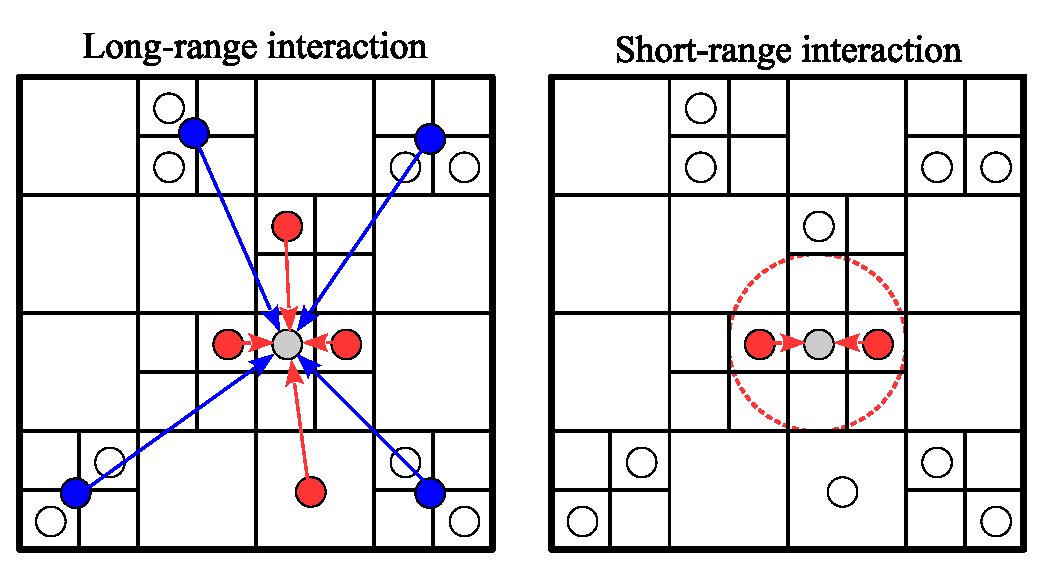
\includegraphics[width=8cm]{force_type.eps}
%  \end{center}
%  \caption{長距離力と短距離力のイメージ図.}
%  \label{fig:force}
%\end{figure}

また,粒子間相互作用の計算において,ある粒子は自分のプロセス以外の粒子
とも相互作用する可能性があるため,FDPS では相互作用に寄与する$j$ 粒子
を通信して相互作用を計算するのに必要な粒子を全て自分のプロセスに集める
方法を採用している.この方法では短距離力の場合は近傍のプロセスと通信す
れば良い.長距離力の場合にはBarnes-Hut tree法を採用しているため,遠く
の計算領域のプロセスからは全ての粒子をもらってくる必要はなく粒子が作る
ポテンシャルの多重極展開の係数を通信すれば十分であり,FDPS もこの方法
を採用している\cite{2004PASJ...56..521M}.

%図\ref{fig:LET} はプロセス間でのj 粒子の通信を表したものである.
%\begin{figure}
%  \begin{center}
%    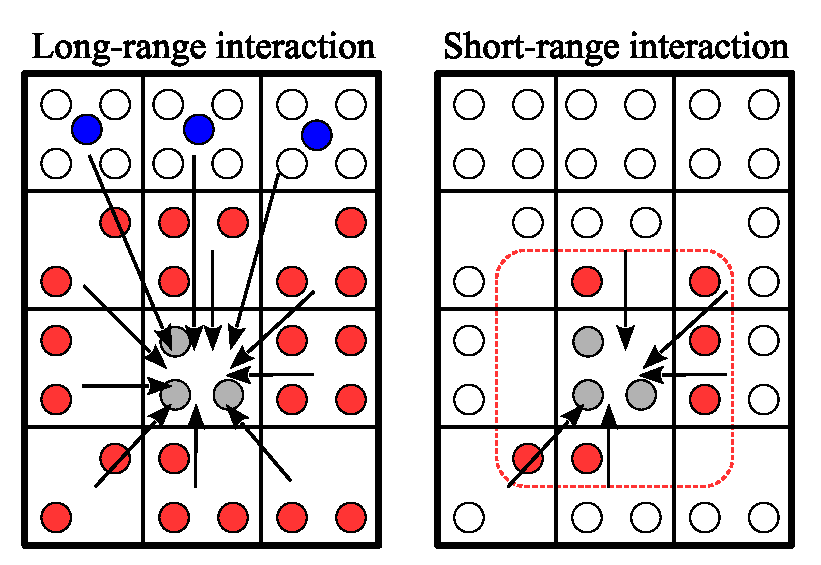
\includegraphics[width=8cm]{exchangeLET.eps}
%  \end{center}
%  \caption{長距離力と短距離力の場合のj粒子交換のイメージ図.}
%  \label{fig:LET}
%\end{figure}

ユーザーがこのクラスのメソッド{\tt
  TreeForForce::calcForceAllAndWriteBack()}を全てのプロセスで呼び出す
と,FDPSは粒子座標から木構造を構築し,相互作用の計算に必要な$j$粒子の
通信を行い,更に相互作用の計算までを行う.この関数内での木構造構築や相
互作用計算はOpenMPにも対応している.

複数種類の相互作用を計算する場合はこのクラスのオブジェクトを複数生成す
れば良い.

%ツリー構造の構築や,ツリー構造を利用した相互作用の計算はプログラム開発
%の困難な部分であるが,この部分についてもFDPSが全て担当しまたOpenMPにも
%対応しているので,ユーザーはこの部分について殆ど意識する必要はない.

%この様に長距離力と短距離力では相互作用を計算するために必要となるj粒子
%が異なるために,j粒子を見つけるためのツリーウォークの方法やまた,他プロセ
%スとのj粒子の通信方法も異なる.そのため,FDPSでは{\tt TreeForForce}クラ
%スのテンプレート引数として,計算する力の週類を入力する事で対処している.


\section{FDPSを用いた重力$N$体シミュレーションコードの実装例}

我々はFDPSのユーザーは以下の流れで粒子系シミュレーションコードの開発を
行う事を想定している。

\begin{enumerate}
\item 粒子のデータ構造をC++のクラスの形で定義する.
\item 相互作用関数をC++の関数テンプレートもしくは関数ポインタの形で定
  義する.相互作用関数は$i$粒子と$j$粒子の配列を受け取り,$i$粒子への相互
  作用を計算し,その結果を積算するように定義する.
\item FDPSによって提供されているデータクラスと関数群を用いてユーザープ
  ログラムを作成する.
\end{enumerate}

図\ref{code:ptcl_class}は重力$N$体シミュレーションの粒子クラスの例
である.

%\begin{lstlisting}[label=code:ptcl_class,numbers=left,numbersep=5pt,frame=single,basicstyle=\ttfamily,caption=粒子データ構造]

\begin{figure}[!h]
\begin{lstlisting}[language=c++,numbers=left,numbersep=5pt,frame=single,basicstyle=\ttfamily]
class Nbody{
public:
  F64    mass, eps;
  F64vec pos, vel, acc;
  F64vec getPos() const {return pos;}
  F64 getCharge() const {return mass;}
  void copyFromFP(const Nbody &in){ 
    mass = in.mass;
    pos  = in.pos;
    eps  = in.eps;
  }
  void copyFromForce(const Nbody &out) {
    acc = out.acc;
  }    
  void clear() {
    acc = 0.0;
  }
};
\end{lstlisting}
\caption{粒子クラス}
\label{code:ptcl_class}
\end{figure}

粒子データクラスの名前やメンバ変数名等は自由であるが,いくつかのメンバ
関数は決まった名前で用意する必要がある(上の例では{\tt getPos()},{\tt
    getCharge()},{\tt copyFromFP()}等).これはその名前を使ってFDPSが
クラス内メンバにアクセスするからである.またメンバ変数の型にある{\tt
  F64}と{\tt F64vec}はFDPSによって定義された型であり,それぞれ64bit浮
動小数点と64bit浮動小数点を成分とする3次元ベクトル型である.ベクトル型
には四則演算や内積外積等のメンバ関数を持っており,ユーザーはこれらを用
いてユーザープログラムを記述することができる.



%\begin{lstlisting}[label=code:force,numbers=left,numbersep=5pt,frame=single,basicstyle=\ttfamily,caption=相互作用関数]

\begin{figure}[!h]
\begin{lstlisting}[language=c++,numbers=left,numbersep=5pt,frame=single,basicstyle=\ttfamily]
struct CalcGrav{
  void operator () (const Nbody * ip,
                    const S32 ni,
                    const Nbody * jp,
                    const S32 nj,
                    Nbody * force) {
    for(S32 i=0; i<ni; i++){
      F64vec xi  = ip[i].pos;
      F64    ep2 = ip[i].eps * ip[i].eps;
      F64vec ai = 0.0;
      for(S32 j=0; j<nj;j++){
        F64vec xj = jp[j].pos;
        F64vec dr = xi - xj;
        F64 mj  = jp[j].mass;
        F64 dr2 = dr * dr + ep2;
        F64 dri = 1.0 / sqrt(dr2);                
        ai -= (dri * dri * dri * mj) * dr;
      }
      force[i].acc += ai;
    }
  }
};
\end{lstlisting}
\caption{相互作用関数}
\label{code:force}
\end{figure}

図\ref{code:force}はニュートン重力の場合の相互作用関数の例である.この
図から分かるように相互作用関数は複数の$i$粒子への複数の$j$粒子からの相
互作用の計算をするものでなくてはならない.ここに出てくる{\tt S32}型は
32bit符号付き整数型である.

\begin{figure}[!h]
\begin{lstlisting}[language=c++,numbers=left,numbersep=5pt,frame=single,basicstyle=\ttfamily]
int main(int argc, char *argv[]) {
  F64 time  = 0.0;
  const F64 tend  = 10.0;
  const F64 dtime = 1.0 / 128.0;
  PS::Initialize(argc, argv);
  PS::DomainInfo dinfo;
  dinfo.initialize();
  PS::ParticleSystem<Nbody> ptcl;
  ptcl.initialize();
  PS::TreeForForceLong<Nbody, Nbody,
      Nbody>::Monopole grav;
  grav.initialize(0);
  ptcl.readParticleAscii(argv[1]);
  while(time < tend) {
    S32 n = p.getNumberOfParticleLocal();
    for(S32 i = 0; i < n; i++)
      ptcl[i].predict(dttime);
    dinfo.decomposeDomainAll(ptcl);
    ptcl.exchangeParticle(dinfo);    
    tree.calcForceAllAndWriteBack
        (CalcGrav<Nbody>(),
         CalcGrav<SPJMonopole>(),
         ptcl, dinfo);    
    n = p.getNumberOfParticleLocal();
    for(S32 i = 0; i < n; i++)
      ptcl[i].correct(dtime);                            
    time += dtime;
  }
  PS::Finalize();
  return 0;
}
\end{lstlisting}
\label{code:main}
\caption{メイン関数}
\end{figure}

図\ref{code:main}はメイン関数の一部である.FDPSの機能を使うためにはま
ず,{\tt PS::Initialize()}を呼ぶ必要がある.6行目で{\tt DomainInfo}ク
ラス,8行目で{\tt ParticleSystem}クラス,10行目で{\tt TreeForForce}ク
ラスのオブジェクトを生成している.ここでは{\tt ParticleSystem}クラスと
{\tt TreeForForce}クラスのテンプレート引数に粒子クラスを与えている.18
行目で担当する計算領域の分割を行い,19行目で粒子の交換を行っている.20
行目では,メソッド{\tt calcForceAllAndWriteBack}の引数に相互作用関数を
与えることで,相互作用の計算を行っている.このプログラムをみて分かる通
り,どこにも明示的にMPIのAPIは呼ばれていない.しかし,このコードはMPI
とOpenMPを用いたハイブリッド並列プログラムとして動く.付録に実際にハイ
ブリッド並列で動作するシンプルな重力$N$体シミュレーションのプログラム
を載せた.このプログラムは120行程で書かれている.

%3
\section{FDPSの内部実装}

この節ではFDPSの提供する関数がどの様に実装されているかを述べる.

\subsection{領域分割と粒子交換}

FDPSでは領域分割にthree-dimensional multi-section法
(MS法)\cite{2004PASJ...56..521M}を採用している.この方法では,最初に計
算領域を$x$軸方向に沿って{\tt nx}個の領域に分割する.次に先ほど分割さ
れた各領域を$y$軸方向に沿って{\tt ny}個の領域に分割する.$z$軸方向につ
いても同様に先ほど分割した領域を$z$軸方向に沿って分割する.領域分割の
方法は他にORB\cite{Blackston:1997:HPE:509593.509597}やモートン順序
\cite{Warren:1993:PHO:169627.169640}によるものが広く使われている.MS法
はORBと違いプロセッサ数が2のべき乗である事を要求せず,任意のプロセッサ
数で動作する.また,モートン順序による領域分割では領域に飛びが出来てし
まう可能性があるがMS法ではそのような事は起こらない.

%図\ref{fig:DD}はこの方法を使って計算領域を(nx,ny,nz)=(7,6,1)に分割した
%場合を表している.

FDPSでは各プロセスが担当する計算領域の座標を求める方法としてサンプリン
グ法\cite{2004PASJ...56..521M}を採用している.この方法では計算領域の位
置座標を各プロセスからサンプリングした粒子のみによって決定する.プロセ
ス数が大きくなるとサンプル数も増えてしまうため,FDPSではこの部分もMPI
を用いた並列化に対応している.また,サンプリングノイズを低減するために,
計算領域の座標に指数移動平均を使うこともできる.

%サンプル数が少な過ぎるとサンプリングノイズが大きくなり,ロードバラン
%スが悪くなってしまうため,あまりサンプル数を減らすことは出来ない.そ
%のためFDPSではこの部分をプロセス並列で計算する事もできるようになって
%いる.また,少ない粒子数でもサンプリングノイズを軽減するように計算領
%域の座標に指数移動平均を使うこともできる.

この様にして計算された計算領域にしたがってプロセス間で粒子の交換を行う.
これは{\tt MPI\_Alltoall}と{\tt MPI\_Isend},{\tt MPI\_Irecv}を用いて
実装されている.


%\begin{figure}
%  \begin{center}
%    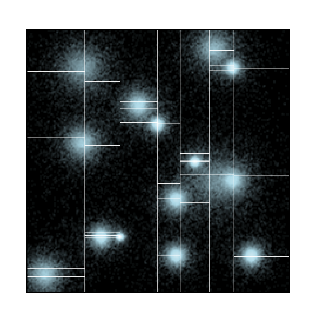
\includegraphics[width=8cm]{pm3d.eps}
%  \end{center}
%  \caption{計算領域を(nx,ny,nz)=(7,6,1)に分割した様子.}
%  \label{fig:DD}
%\end{figure}

\subsection{相互作用計算}

この節では,相互作用の計算の内部実装について述べる.まず,{\tt
  TreeForForce}クラスは{\tt ParticleSystem}クラスから相互作用計算を行
うために必要な粒子のデータを受け取り内部に保持する.この粒子データから
八分木構造を作り粒子を管理する.八分木構造の作り方は以下の様になってい
る.

\begin{enumerate}
\item 各粒子のモートン鍵を計算する.
\item 基数ソートを使ってモートン鍵の順番に粒子を並べる.
\item 木構造を階層ごとに上から作っていく.モートン鍵の上位3bitをみて各
  粒子の対応するツリーセルを見つける.この際粒子はソートされているため
  バイナリーサーチを使うことができる.
\end{enumerate}

FDPSではこの全ての手順をOpenMP化している.

次にこの木構造を利用して相互作用を計算するために必要な粒子の交換を行う.
短距離力の場合は近傍の計算領域を担当するプロセスとだけ通信を行えば良い.
これは{\tt MPI\_Isend}と{\tt MPI\_Irecv}を使って実装されている.長距離
力の場合は各プロセッサから送られてくるメッセージサイズは比較的小さいが
全体全の通信が必要になる.これは{\tt MPI\_Alltoall(v)}により実装されて
いる.しかし,「京」コンピュータの場合は短いメッセージ長の{\tt
  MPI\_Alltoall(v)}はあまり最適化がなされていないため,メッセージの数
を減らす様に同じ中継ポイントにいくメッセージを統合する方式をとっている.

送られてきた粒子情報から先ほどと同じ方法で再び木構造を構築する.この木
構造を用いて$j$粒子の探索を行う.ここでは,局所的にまとめた$i$粒子の集
団に対して$j$粒子の探索を行い、ユーザーの定義した相互作用関数にしたっ
がって相互作用を計算する.FDPSではOpenMPを用いて$j$粒子探査と相互作用
の計算をスレッド並列化している.

%4
\section{性能}

%この節ではFDPSを使って開発した2つのアプリケーションプログラムの性能と
%プログラムの大きさについて述べる.この節で行ったシミュレーションは全て
%「京」を使って行った.

この節ではFDPSを使って開発した2つのアプリケーションプログラムの性能に
ついて述べる.この節で行ったシミュレーションは全て「京」を使って行った.
このシミュレーションでの並列化方法はノード内についてはOpenMPを使い,ノー
ド間についてはMPIを用いたハイブリッド並列である.

\subsection{アプリケーション・プログラムの性能}

%4.1
\subsubsection{重力N体シミュレーション}

本節ではFDPSを用いた重力$N$体コードの性能を述べる.

ここで使ったプログラムは前の節で述べ,付録に掲載されているプログラムと
本質的には同じであるが,1つ大きな違いがある.ここでは,前の節の相互作
用関数と違い高度に最適化された相互作用関数を使っている.

本シミュレーションでは,初期モデルとして,星団や銀河のシミュレーション
で広く使われている力学平衡モデルの一つであるプラマーモデル
\cite{1911MNRAS..71..460P}を用いた.重力の計算にはツリーの見込み角
$\theta = 0.4$として,四重極子までの展開を使った.

図\ref{fig:bench}は1プロセス当たりの平均の粒子数を約210万体とした場合
の速度(上図)と1ステップ当たりのウォールクロックタイム(下図)をプロセス
数の関数としてプロットしたものである.非常に良くスケールしている事が分
かる.実行効率も理論ピーク性能の50\%を達成している.

\begin{figure}[!h]
  \begin{center}
    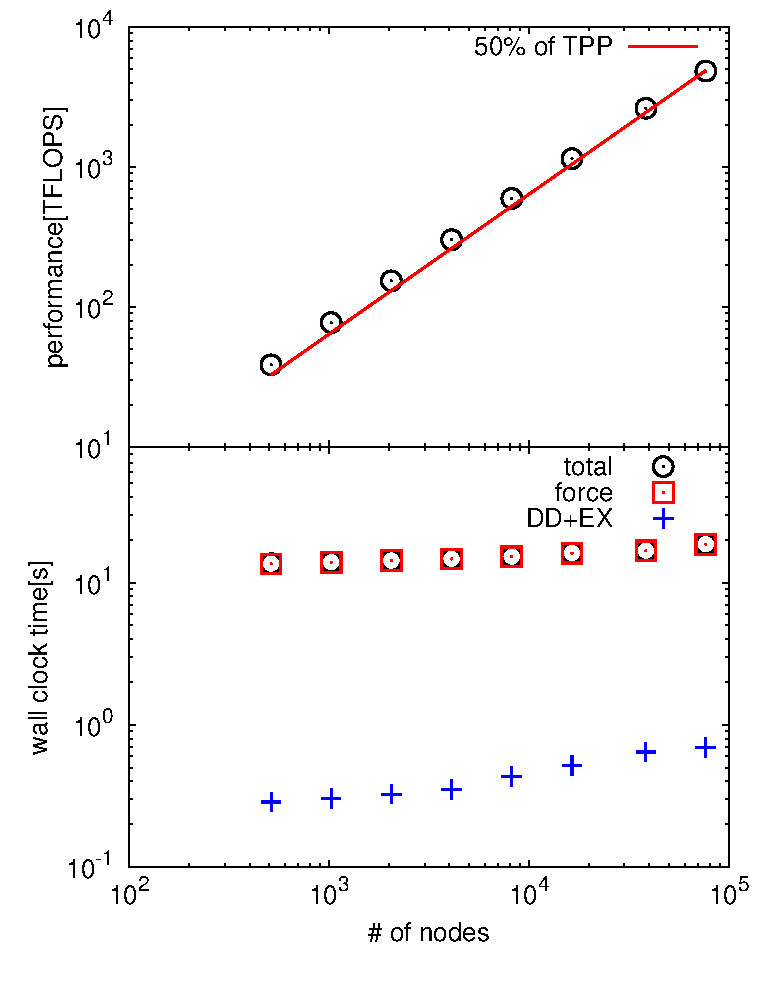
\includegraphics[width=8cm]{bench_nbody.eps}
  \end{center}
  \caption{重力$N$体シミュレーションでの性能.上:黒丸は本アプリケショ
    ンの速度であり,赤線は理論ピーク性能の50\%を表している.下:黒丸は
    計算時間の合計,赤四角は重力の計算にかかった時間,青十字は領域分割
    と粒子交換にかかった時間の合計を表している.}
  \label{fig:bench}
\end{figure}

%4.2
\subsubsection{SPHシミュレーション}

本節ではFDPSを用いたSPH法での性能を述べる.

我々はSPH法のシミュレーションとして,月形成の有力なシナリオである巨大
衝突仮説\cite{1976LPI.....7..120C,1975Icar...24..504H}のシミュレーショ
ンを行った.巨大衝突仮説とは50億年程前に火星サイズの天体が原始地球に衝
突しその際に撒き散らされた破片が集積し月になったとする説である.多くの
研究者によって巨大衝突シミュレーションが行われている
\cite{1986Icar...66..515B,2013Icar..222..200C,2014NatGe...7..564A}.

重力の計算にはツリーの見込み角$\theta = 0.5$として,単極子までの展開を
使った.流体部分の計算は標準SPH法を使った
\cite{1997JCoPh.136..298M,2009NewAR..53...78R,2010ARA&A..48..391S}.

図\ref{fig:bench_gi}は1プロセス当たりの平均の粒子数を約31万体とした場
合の速度(上図)と1ステップ当たりのウォールクロックタイム(下図)をプロセ
ス数の関数としてプロットしたものである.本シミュレーションも良くスケー
ルしている事が分かる.実行効率も理論ピーク性能の40\%程度を達成している.
図から重力の計算に比べて,流体の計算にかかる時間が大きい事が分かる.こ
れは流体の1相互作用当たりの計算量は重力相互作用のそれに比べて非常に大
きいためである.

\begin{figure}[!h]
  \begin{center}
    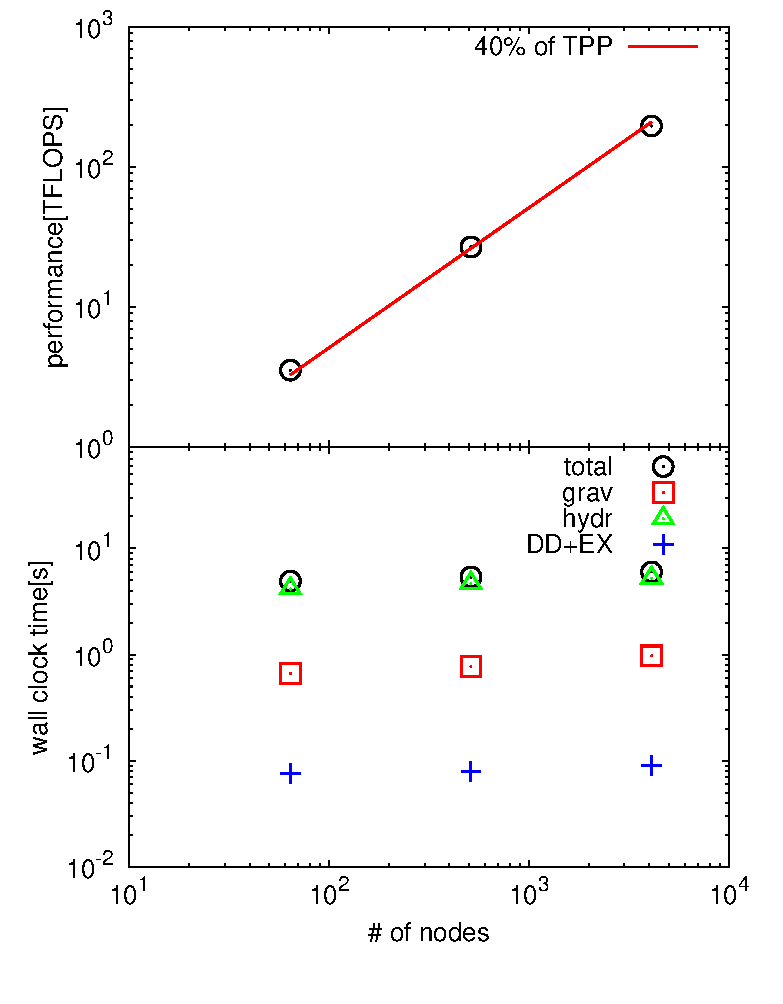
\includegraphics[width=8cm]{bench_gi.eps}
  \end{center}
  \caption{巨大衝突シミュレーションの性能.上:黒丸は本アプリケションの
    速度であり,赤線は理論ピーク性能の40\%を表している.下:黒丸は計算
    時間の合計,赤四角は重力の計算にかかった時間,緑三角は流体の密度と
    面積力を求めるのにかかった時間,青十字は領域分割と粒子交換にかかっ
    た時間の合計を表している.}
  \label{fig:bench_gi}
\end{figure}

\section{外部モジュール}

FDPSでは有用ないくつかの外部モジュールも提供している.その一つは
Particle-Mesh法により力を計算するモジュールである.これは
GreeM\cite{ishiyama:greem,ishiyama:gordonbell}で使われている
Particle-Mesh法のモジュールをFDPS用にラップしたものである.これにより,
ユーザーはPPPM法やPMTree法\cite{2005PASJ...57..849Y}のプログラムを容易
に開発できる.また,他の外部モジュールとしては高度に最適化されたニュー
トン重力の計算を実行するライブラリが用意されている
\cite{2006NewA...12..169N,2012NewA...17...82T,2013NewA...19...74T}.

外部モジュールは今後も開発していく予定である.



%\subsection{ソースコードの大きさ}

%本節では上の2つのシミュレーションで使用したソースコードの行数について
%述べる.

%表\ref{tab:applicationsize}は上で行った2つのシミュレーションのソース
%コード行数を項目別に示した.どちらも相互作用関数の定義が長くなっている
%事が分かる,これはSIMDユニットを有効に利用するために「京」の組み込み関
%数を使った事また,手動でループ展開等も行ったためである.

%\begin{table}
%  \begin{center}
%  \caption{ソースコードの行数}
%  \label{tab:applicationsize}
%  \begin{tabular}{lcc}
%    \hline
%      & 重力$N$体 & SPH\\
%    \hline
%    合計 & 801 & 1298 \\
%    粒子データ定義 &  51 & 226 \\
%    相互作用関数 &  437 & 570 \\
%    初期条件設定と I/O &  128 & 96 \\
%    積分ループ &  12 & 49 \\
%    その他 & 173 & 357\\
%\hline    
%  \end{tabular}
%  \end{center}
%\end{table}

%リストは本シミュレーションで使用した相互作用関数定義の一部である.




%5
\section{まとめ}

我々は大規模並列粒子法シミュレーションプログラム開発を容易にするフレー
ムワークFDPSの開発を行った.FDPSを使う事でユーザーは並列化を意識するこ
となく,容易にソフトウェア開発をできるようになった.また,実際にFDPSを
用いた2つのアプリケーション・プログラム(重力N体シミュレーションコード
  とSPHシミュレーションコード)の開発を行い,性能,スケーラビリティー
を測定した.結果,両アプリケーション共に,非常に高い実行性能で動作する
ことが分かった.


\begin{acknowledgment}
  外部モジュールとしてPMTreeコードを提供して下さった石山智明氏,ユーザー
  の立場から多大な助言をして下さった丸山豊氏,本プロジェクト全体の管理
  をして下さった坪内美幸氏に感謝します.
\end{acknowledgment}

\bibliography{ms}

%\begin{thebibliography}{10}
%\bibitem{okumura}
%奥村晴彦:改訂第5版 \LaTeXe 美文書作成入門,
%技術評論社(2010).
%\end{thebibliography}

\appendix

\section{重力$N$体シミュレーションサンプルコード}

\begin{lstlisting}[language=c++,label=code:samplecode,numbers=left,numbersep=5pt,frame=single,basicstyle=\ttfamily]
#include <particle_simulator.hpp>
using namespace PS;
class Nbody{
public:
  F64    mass, eps;
  F64vec pos, vel, acc;
  F64vec getPos() const {return pos;}
  F64 getCharge() const {return mass;}
  void copyFromFP(const Nbody &in){ 
    mass = in.mass;
    pos  = in.pos;
    eps  = in.eps;
  }
  void copyFromForce(const Nbody &out) {
    acc = out.acc;
  }    
  void clear() {
    acc = 0.0;
  }
  void readAscii(FILE *fp) {
    fscanf(fp,
           "%lf%lf%lf%lf%lf%lf%lf%lf",
           &mass, &eps,
           &pos.x, &pos.y, &pos.z,
           &vel.x, &vel.y, &vel.z);
  }
  void predict(F64 dt) {
    vel += (0.5 * dt) * acc;
    pos += dt * vel;
  }
  void correct(F64 dt) {
    vel += (0.5 * dt) * acc;
  }
};

template <class TPJ>
struct CalcGrav{
  void operator () (const Nbody * ip,
                    const S32 ni,
                    const TPJ * jp,
                    const S32 nj,
                    Nbody * force) {
    for(S32 i=0; i<ni; i++){
      F64vec xi  = ip[i].pos;
      F64    ep2 = ip[i].eps
          * ip[i].eps;
      F64vec ai = 0.0;
      for(S32 j=0; j<nj;j++){
        F64vec xj = jp[j].pos;
        F64vec dr = xi - xj;
        F64 mj  = jp[j].mass;
        F64 dr2 = dr * dr + ep2;
        F64 dri = 1.0 / sqrt(dr2);                
        ai -= (dri * dri * dri
               * mj) * dr;
      }
     force[i].acc += ai;
    }
  }
};

template<class Tpsys>
void predict(Tpsys &p,
             const F64 dt) {
  S32 n = p.getNumberOfParticleLocal();
  for(S32 i = 0; i < n; i++)
    p[i].predict(dt);
}

template<class Tpsys>
void correct(Tpsys &p,
             const F64 dt) {
  S32 n = p.getNumberOfParticleLocal();
  for(S32 i = 0; i < n; i++)
    p[i].correct(dt);
}

template<class TDI, class TPS,
         class TTF>
void calcGravAllAndWriteBack(TDI &dinfo,
                             TPS &ptcl,
                             TTF &tree){
  dinfo.decomposeDomainAll(ptcl);
  ptcl.exchangeParticle(dinfo);    
  tree.calcForceAllAndWriteBack
    (CalcGrav<Nbody>(),
     CalcGrav<SPJMonopole>(),
     ptcl, dinfo);    
}

int main(int argc, char *argv[]) {
  F32 time  = 0.0;
  const F32 tend  = 10.0;
  const F32 dtime = 1.0 / 128.0;
  PS::Initialize(argc, argv);
  PS::DomainInfo dinfo;
  dinfo.initialize();
  PS::ParticleSystem<Nbody> ptcl;
  ptcl.initialize();
  PS::TreeForForceLong<Nbody, Nbody,
      Nbody>::Monopole grav;
  grav.initialize(0);
  ptcl.readParticleAscii(argv[1]);
  calcGravAllAndWriteBack(dinfo,
                          ptcl,
                          grav);
  while(time < tend) {
    predict(ptcl, dtime);        
    calcGravAllAndWriteBack(dinfo,
                            ptcl,
                            grav);
    correct(ptcl, dtime);        
    time += dtime;
  }
  PS::Finalize();
  return 0;
}
\end{lstlisting}

%\label{code:sample}
%\caption{重力$N$体シミュレーション用サンプルコード}
%\end{figure}

%\begin{biography}
%\profile{m}{情報 太郎}{1970年生.1992年情報処理大学理学部情報科学科卒.
%1994年同大大学院修士課程了.同年情報処理学会入社.オンライン出版の研究
%に従事.電子情報通信学会,IEEE,ACM 各会員}
%\end{biography}



\end{document}
